\newpage
\section{Problem E - a+b问题}
{ \limitfont{}
Input file: standard input \par
Output file: standard output \par
Time limit: 1000ms \par
Memory limit: 64MB \par
}

\subsection*{题目描述}

ml 喜欢吃彩虹糖、棒棒糖和巧克力糖。但是 ml 花了太多钱请漂亮姐姐吃饭而变得贫穷,所以 ml 只能每 $b_1$ 天买一次彩虹糖,每 $b_2$ 天买一次棒棒糖,每 $b_3$ 天买一次巧克力糖。注意:买 $3$ 种糖是独立进行的,ml 并没有贫穷到需要思索要买哪一种糖。

\begin{figure}[H]
    \centering
    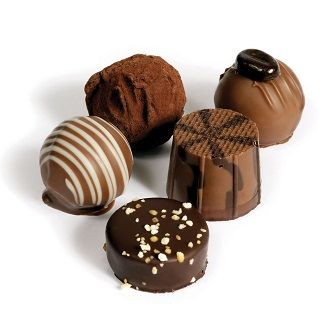
\includegraphics[scale=0.5]{./src/e.png}
\end{figure}

ml 希望有一种策略,使得 ml 每天都能吃到糖(即彩虹糖,棒棒糖,巧克力糖其中一种或者多种)。

准确地,ml 会选择 $a_1,a_2,a_3$ 分别做为第一次购买彩虹糖、棒棒糖和巧克力糖的日期,这样他在第 $a_1,a_1+b_1,a_1+2b_1,a_1+3b_1,\dots$ 天会购买彩虹糖;在第 $a_2,a_2+b_2,a_2+2b_2,a_2+3b_2,\dots$ 天会购买棒棒糖;在第 $a_3,a_3+b_3,a_3+2b_3,a_3+3b_3,\dots$ 天会购买巧克力糖。

请问是否存在一组 $a_1,a_2,a_3$ 使得 ml 从某一天开始,每天都能吃到糖;存在输出 ``YES'',不存在则输出 ``NO''。

\subsection*{输入描述}

输入一行,包括三个正整数 $b_1,b_2,b_3$($1\leq b_1,b_2,b_3\leq 1000$),使用空格分隔。

\subsection*{输出描述}

输出 ``YES'' 或者 ``NO''。

\subsection*{测试样例}

\begin{table}[H]
\begin{tabularx}{\textwidth}{|X|X|}
    \hline
    \textbf{Standard Input} & \textbf{Standard Output} \\ 
    \hline 
    \tablecell{
        1 1 1 \\
    } & 
    \tablecell{YES \\} \\
    \hline
    \tablecell{
        2 2 2 \\
    } & \tablecell{
        YES \\
    } \\
    \hline
    \tablecell{
        3 3 3 \\
    } & \tablecell{
        YES \\
    } \\
    \hline
    \tablecell{
        2 3 4 \\
    } & \tablecell{
        NO
    } \\
    \hline
\end{tabularx}
\end{table}
    